\documentclass{standalone}

\usepackage{libertinus}
\usepackage[T1]{fontenc}
\renewcommand*\familydefault{\sfdefault}

\usepackage{DejaVuSansMono}

\usepackage{tikz}
\usetikzlibrary{decorations.pathmorphing, decorations.pathreplacing, decorations.shapes}
\tikzset{every path/.style={semithick}}

\newcommand{\queues}[2]{
  \draw[->,decorate,decoration=zigzag] (#1+1,#2+0.18) -- (#1+1,#2+1);
  \draw[<-] (#1+1,#2) -- ++(0,0.19);
}

\begin{document}
  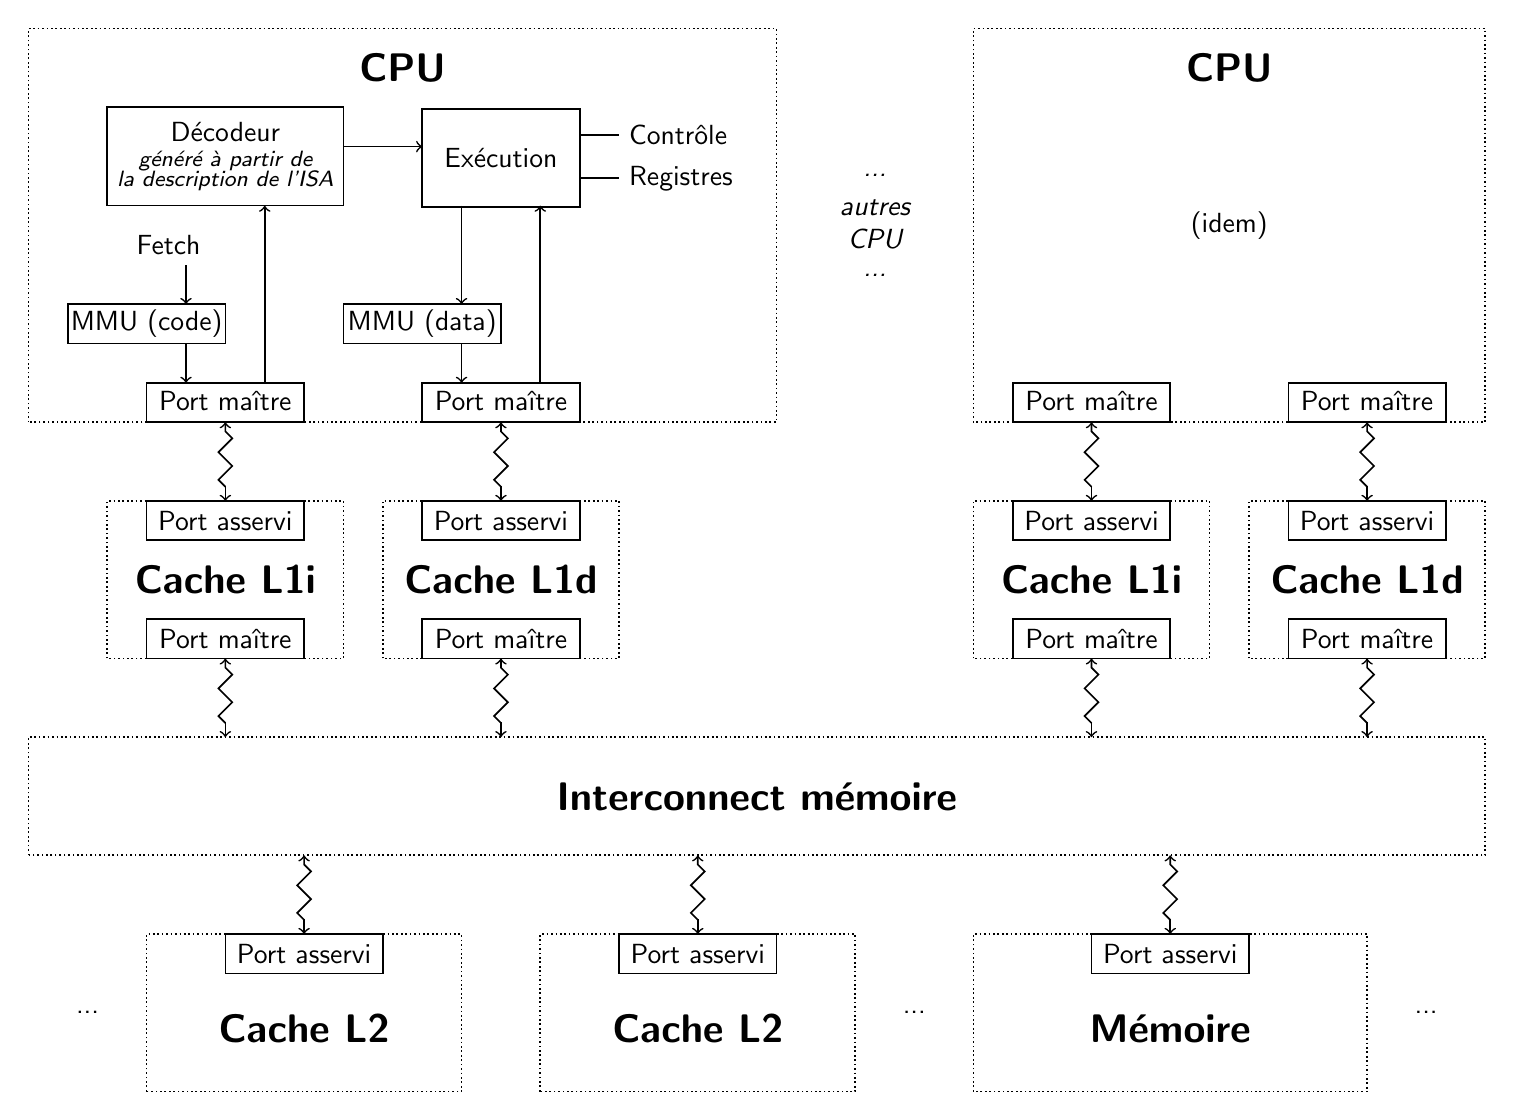
\begin{tikzpicture}
    % CPU 1

    \begin{scope}[shift={(0,0)}]
      \draw (0.5,0) rectangle node[text depth=0.3ex] {Port maître} ++(2,0.5);
      \draw (-0.5,1) rectangle node {MMU (code)} ++(2,0.5);
      \draw[<-] (1,0.5) -- ++(0,0.5);
      \draw[<-] (1,1.5) -- ++(0,0.5) node [above left, xshift=2ex] {Fetch};
      \draw (0,2.75) rectangle node[align=center] {Décodeur \\[-3pt] \footnotesize\it généré à partir de \\[-5pt] \footnotesize\it la description de l'ISA} ++(3,1.25);
      \draw[->] (2,0.5) -- ++(0,2.25);

      \draw[->] (3,3.5) -- (4,3.5);
      \draw (4,2.73) rectangle node {Exécution} ++(2,1.25);
      \draw (6,3.1) -- ++(0.5, 0) node[right] {Registres};
      \draw (6,3.65) -- ++(0.5, 0) node[right] {Contrôle};

      \draw[->] (4.5,2.75) -- ++(0,-1.25);

      \draw (4,0) rectangle node[text depth=0.3ex] {Port maître} ++(2,0.5);
      \draw (3,1) rectangle node {MMU (data)} ++(2,0.5);
      \draw[<-] (4.5,0.5) -- ++(0,0.5);
      \draw[->] (5.5,0.5) -- ++(0,2.25);

      \draw[densely dotted] (-1, 0) rectangle (8.5,5);
      \draw (3.75, 4.5) node {{\bf\Large CPU}};
    \end{scope}

    \queues{0.5}{-1}
    \begin{scope}[shift={(0,-3)}]
      \draw[densely dotted] (0,0) rectangle ++(3, 2);
      \draw (0.5,1.5) rectangle node {Port asservi} ++(2,0.5);
      \draw (1.5,1)  node {{\bf\Large Cache L1i}};
      \draw (0.5,0) rectangle node {Port maître} ++(2,0.5);
    \end{scope}

    \queues{4}{-1}
    \begin{scope}[shift={(3.5,-3)}]
      \draw[densely dotted] (0,0) rectangle ++(3, 2);
      \draw (0.5,1.5) rectangle node {Port asservi} ++(2,0.5);
      \draw (1.5,1)  node {{\bf\Large Cache L1d}};
      \draw (0.5,0) rectangle node {Port maître} ++(2,0.5);
    \end{scope}

    % CPU 2

    \begin{scope}[shift={(12,0)}]
      \draw (-0.5,0) rectangle node[text depth=0.3ex] {Port maître} ++(2,0.5);
      \draw (3,0) rectangle node[text depth=0.3ex] {Port maître} ++(2,0.5);

      \draw[densely dotted] (-1, 0) rectangle node {(idem)} (5.5,5);
      \draw (2.25, 4.5) node {{\bf\Large CPU}};
    \end{scope}

    \queues{11.5}{-1}
    \begin{scope}[shift={(11,-3)}]
      \draw[densely dotted] (0,0) rectangle ++(3, 2);
      \draw (0.5,1.5) rectangle node {Port asservi} ++(2,0.5);
      \draw (1.5,1)  node {{\bf\Large Cache L1i}};
      \draw (0.5,0) rectangle node {Port maître} ++(2,0.5);
    \end{scope}

    \queues{15}{-1}
    \begin{scope}[shift={(14.5,-3)}]
      \draw[densely dotted] (0,0) rectangle ++(3, 2);
      \draw (0.5,1.5) rectangle node {Port asservi} ++(2,0.5);
      \draw (1.5,1)  node {{\bf\Large Cache L1d}};
      \draw (0.5,0) rectangle node {Port maître} ++(2,0.5);
    \end{scope}

    % Autres

    \draw (9.75, 2.5) node[align=center,font=\it] {... \\[2pt] autres \\ CPU \\[-2pt] ...};

    \queues{0.5}{-4}
    \queues{4}{-4}
    \queues{11.5}{-4}
    \queues{15}{-4}
    \draw[densely dotted] (-1,-5.5) rectangle node {\bf\Large Interconnect mémoire} ++(18.5, 1.5);

    \begin{scope}[shift={(1,-8.5)}]
      \queues{0.5}{2}
      \draw[densely dotted] (-0.5,0) rectangle ++(4, 2);
      \draw (0.5,1.5) rectangle node {Port asservi} ++(2,0.5);
      \draw (1.5,0.8)  node {{\bf\Large Cache L2}};
    \end{scope}

    \begin{scope}[shift={(6,-8.5)}]
      \queues{0.5}{2}
      \draw[densely dotted] (-0.5,0) rectangle ++(4, 2);
      \draw (0.5,1.5) rectangle node {Port asservi} ++(2,0.5);
      \draw (1.5,0.8)  node {{\bf\Large Cache L2}};
    \end{scope}

    \begin{scope}[shift={(12,-8.5)}]
      \queues{0.5}{2}
      \draw[densely dotted] (-1,0) rectangle ++(5, 2);
      \draw (0.5,1.5) rectangle node {Port asservi} ++(2,0.5);
      \draw (1.5,0.8)  node {{\bf\Large Mémoire}};
    \end{scope}

    \draw (-0.25,-7.5) node {...};
    \draw (10.25,-7.5) node {...};
    \draw (16.75,-7.5) node {...};
  \end{tikzpicture}
\end{document}
